\documentclass[runningheads]{llncs}
%

%\usepackage{amsmath}
\usepackage{amssymb}
%\usepackage{amsthm}


\usepackage{graphicx}


% Used for displaying a sample figure. If possible, figure files should
% be included in EPS format.
%
% If you use the hyperref package, please uncomment the following line
% to display URLs in blue roman font according to Springer's eBook style:
% \renewcommand\UrlFont{\color{blue}\rmfamily}

\newcommand{\tup}[1]{{\langle #1 \rangle}}
\newcommand{\pre}{\mathsf{pre}}    % precondition
\newcommand{\eff}{\mathsf{eff}}    % effect
\newcommand{\cond}{\mathsf{cond}}  % condition
\newcommand{\dur}{\mathsf{dur}}    % duration
\newcommand{\obs}{\mathsf{obs}}    % observation
\newcommand{\start}{\mathsf{start}}% start
\newcommand{\en}{\mathsf{end}}     % end
\newcommand{\til}{\mathsf{til}}    % TIL
\newcommand{\supp}{\mathsf{sup}}   % sup
\newcommand{\tim}{\mathsf{time}}   % time
\newcommand{\reqs}{\mathsf{req\_{start}}} % req_start
\newcommand{\reqe}{\mathsf{req\_{end}}}   % req_end
\newcommand{\ini}{\mathsf{init}}   % init
\newcommand{\goal}{\mathsf{goal}}  % goal
%\newcommand{\add}{\mathsf{add}}
%\newcommand{\del}{\mathsf{del}}



\begin{document}

\title{One-Shot Learning of Temporal Action Models with Constraint Programming}
%\title{On the Application of Constraint Programming for One-Shot Learning Temporal Planning Models\thanks{This work is supported by the Spanish...}}


\titlerunning{Learning of Temporal Action Models with CP}
% If the paper title is too long for the running head, you can set
% an abbreviated paper title here
%
%\author{Antonio Garrido \and Sergio Jim\'enez}

%\authorrunning{A. Garrido, S. Jim\'enez}
% First names are abbreviated in the running head.
% If there are more than two authors, 'et al.' is used.
%
%\institute{Universitat Polit\`ecnica de Val\`encia \\ Camino de Vera s/n. 46022 Valencia, Spain
%\\ \email{\{agarridot,serjice\}@dsic.upv.es}}

\maketitle              % typeset the header of the contribution

\begin{abstract}
This work proposes a novel constraint programming approach for learning durative actions in an expressive temporal planning model with overlapping actions, which makes it suitable for learning in multi-agent environments.
We analyze the extreme scenario, where just a single (one-shot) partial observation of the execution of a temporal plan is available, to learn the distribution of conditions/effects and estimate the durations, resulting in a consistent constraint model.
Our approach automatically builds a purely declarative formulation that models time-stamps for actions, causal link relationships (conditions and effects), threats and effect interferences that appear in planning. It also accommodates a different range of expressiveness, subsuming the PDDL2.1 temporal semantics. Our formulation is simple but effective, and is not only valid for learning, but also for plan validation, as shown in its evaluation that returns high success ratios. Finally, our formulation is solver-independent, meaning that an arbitrary CSP solver can be used for its resolution.


%Otros titulos:  Learning Temporal Planning Models from Partial Observability by using Constraint Programming; On the Application of Constraint Programming to Learning and Validating;
%Learning Temporal Planning Models from Partial Observability of Plan Executions

%The paper shows that existing CSP compilations for temporal planning can be adapted to build action models for temporal planning.


%150--250 words.

%3 Mayo abstract
%10 mayo full paper 15 pages (references not included)
%Paper: 15 pages

%Application track - scheduling, rostering and planning;
%Incluso en Testing and Verification como segunda opción

\keywords{One-shot learning action models \and Temporal planning \and Partial observability \and Constraint programming.}
\end{abstract}


\section{Introduction}
\label{sec:introduction}

{\em Automated planning} is the model-based approach for the task of selecting the actions that achieve a given set of goals starting from a given initial state. {\em Classical planning} is the vanilla model for planning and it assumes: fully observable states under a deterministic world, instantaneous actions, and goals that are exclusively referred to the last state reached by a plan~\cite{geffner2013concise,ghallab2004automated}. Beyond classical planning, there is a bunch of more expressive planning models that relax the previous assumptions to compute more detailed solutions than classical plans~\cite{ghallab2004automated}.

{\em Temporal planning} is one of these more expressive planning models, as it relaxes the assumption of instantaneous actions~\cite{fox2003pddl2}. Temporal actions have durations and conditions/effects that must hold/happen at different times, which means that temporal actions can be executed in parallel and overlap in several ways~\cite{cushing2007temporal}. Consequently, valid solution plans for temporal planning problems need to indicate the precise time-stamp when an action starts and ends~\cite{howey2004val}.

Despite the potential of state-of-the-art planners, its applicability to the real world is still somewhat limited because of the difficulty of specifying correct and complete planning models~\cite{kambhampati2007model}. The more expressive the planning model is, the more evident becomes this knowledge acquisition bottleneck, which jeopardizes the usability of AI planning technology. This has led to a growing interest in the planning community for the learning of action models~\cite{jimenez2012review}. The objective of this learning task is to compute the actions' conditions and effects that are {\em consistent} with a set of noiseless observations (defined as some sequence of state changes, input constraints,
%world transitions,
expert demonstrations or plan traces/logs). Model learning from observation of past behavior provides indirect, but very valuable information to hypothesize the action models, thus helping future planning decisions and recommendations. This is specially interesting for proactive assistants when recognizing activities of multiple (human or software) agents to assist them in their daily activities.
% and, as the last frontier, to predict and anticipate their needs or actions.

Most approaches for learning planning action models are purely inductive and often require large datasets of observations, e.g. thousands of plan observations to compute a statistically significant model that minimizes some error metric over the observations~\cite{kuvcera2018louga,MouraoZPS12,yang2007learning,zhuo2013action}. Defining model learning as an optimization task over a set of observations does not guarantee completeness (the learned model may fail to explain an observation), nor correctness (the states induced by the execution of the plan generated with the model may contain contradictory information). This paper analyzes the application of Constraint Programming for {\em one-shot learning} of temporal action models, that is, the extreme case of learning action models from a single and partially specified model observed from the execution of a temporal plan. Further, the paper evidences that the learning of action models strongly resembles the task of synthesizing and validating a plan that satisfies all the imposed constraints or, in other words, that is consistent with the noiseless input observations.


While learning an action model for classical planning means computing the actions' conditions and effects that are consistent with the input observations, learning temporal action models extends this to: i) identify how these conditions and effects are temporally distributed in the action execution, and ii) estimate the action duration. As a motivating example, let us assume a logistics scenario. Learning the temporal planning model will allow us: i) to better understand the insights of the logistics in terms of what is possible (or not) and why, because the model is consistent with the observed data; ii) to suggest changes that can improve the model originally created by a human, e.g. re-distributing the actions' conditions, provided they still explain the observations; and iii) to automatically elaborate
similar models for similar scenarios, such as public transit for commuters, tourists or people in general in metropolitan areas ---\emph{a.k.a.} smart urban mobility.


Learning classical action models has been addressed by different approaches~\cite{arora2018review}. Since pioneering learning systems like ARMS~\cite{yang2007learning}, we have seen systems able to learn action models with quantifiers~\cite{AmirC08,ZhuoYHL10}, from noisy actions or states~\cite{MouraoZPS12,zhuo2013action}, from null state information~\cite{cresswell2013acquiring}, or from incomplete domain models~\cite{ZhuoK17,ZhuoNK13}. But, to our knowledge, none of these systems learns the temporal features. This means that observations may now refer to the execution of overlapping durative actions, which makes our approach suitable for learning in multi-agent environments.



\section{Background and Terminology}
\label{sec:background}

This section formalizes the {\em classical} and {\em temporal} planning models that we follow in this work.


\subsection{Classical Planning}
\label{sec:classicalplanning}


Let $F$ be a set of facts that represent propositional variables.
%Without loss of generality, we assume that $F$ does not contain conflicting values $f$ and $\neg f$.
A state $s$ is a full assignment of values to variables, $|s|=|F|$, so the size of the state space is $2^{|F|}$.
A {\em classical planning problem} is a tuple $\tup{F,I,G,A}$, where $I$ is the initial state, $G \subseteq F$ is a set of goal conditions over $F$, and $A$ is the set of actions that modify states. We assume that actions are grounded from action schemas or operators, as in PDDL (Planning Domain Definition Language~\cite{fox2003pddl2,ghallab2004automated}).

Each action $a \in A$ has a set of preconditions $\pre(a)$ and a set of effects $\eff(a)$; $\pre(a), \eff(a) \subseteq F$. $\pre(a)$ must hold before $a$ starts (this is why they are named \emph{pre}conditions), whereas $\eff(a)$ happen when $a$ ends. This way, $a$ is applicable in a state $s$ if $\pre(a) \subseteq s$. When $a$ is executed, a new state, the successor of $s$, is created that results of applying $\eff(a)$ on $s$. Typically, $\eff(a)$ is formed by positive and negative/delete effects. Fig.~\ref{fig:exampleactions1} shows an example of two classical actions for a logistics scenario, from the \emph{driverlog} domain of the International Planning Competition.\footnote{IPC, \texttt{http://www.icaps-conference.org/index.php/Main/Competitions}} Action \texttt{board-truck} boards a driver on an empty truck at a given location. In \texttt{drive-truck} a truck is driven between two locations, provided there is a link between them.

\begin{figure}
\begin{tabular}{p{\textwidth}}
\begin{verbatim}
(:action board-truck
  :parameters (?d - driver ?t - truck ?l - location)
  :precondition (and (at ?d ?l) (empty ?t) (at ?t ?l) )
  :effect (and (not (at ?d ?l)) (not (empty ?t)) (driving ?d ?t)))

(:action drive-truck
  :parameters (?t - truck ?from - location ?to - location ?d - driver)
  :precondition (and (at ?t ?from) (link ?from ?to) (driving ?d ?t))
  :effect (and (not (at ?t ?from)) (at ?t ?to)))
\end{verbatim}
\end{tabular}
\caption{\small PDDL schema for two classical actions from the {\em driverlog} domain.}
\label{fig:exampleactions1}
\end{figure}


In this work we define a plan for a classical planning problem as a set of pairs $\tup{(a_1,t_1),(a_2,t_2)\ldots (a_n,t_n)}$. Each $(a_i,t_i)$ pair contains an instantaneous action $a_i$ and the planning step $t_i$ when $a_i$ starts.
This action sequence induces a state sequence $\tup{s_1,s_2\ldots s_n}$, where each $a_i$ is applicable in $s_{i-1}$, being $s_0=I$, and generates state $s_i$. In every valid plan $G\subseteq s_n$, i.e. the goal condition is satisfied in the last state.
In general terms, classical plans can be sequential plans, where only one action is executed at each planning step, or parallel plans, where several actions can be executed at the same planning step.




\subsection{Temporal Planning}
\label{sec:temporalplanning}

A {\em temporal planning problem} is also a tuple $\tup{F,I,G,A}$ where $F$, $I$ and $G$ are defined like in classical planning, and $A$ represents the set of {\em durative actions}. There are several options that allow for a high expressiveness of durative actions. On the one hand, an action can have a fixed duration, a duration that ranges within an interval or a distribution of durations. On the other hand, actions may have conditions/effects at different times, such as conditions that must hold some time before the action starts, effects that happen just when the action starts, in the middle of the action or some time after the action finishes~\cite{garrido2009constraint}.

A popular model for temporal planning is given by PDDL2.1~\cite{fox2003pddl2}, a language that somewhat restricts temporal expressiveness, which defines a durative action $a$ with the following elements:

\begin{itemize}

\item $\dur(a)$, a positive value for the action duration.

\item $\cond_s(a), \cond_o(a), \cond_e(a) \subseteq F$. Unlike the \emph{pre}conditions of a classical action, now conditions must hold before $a$ ({\em at start}), during the entire execution of $a$ ({\em over all}) or when $a$ finishes ({\em at end}), respectively. In the simplest case, $\cond_s(a) \cup \cond_o(a) \cup \cond_e(a) = \pre(a).$\footnote{Note that in classical planning, $\pre(a)=\{p,not-p\}$ is contradictory. In temporal planning, $\cond_s(a)=\{p\}$ and $\cond_e(a)=\{not-p\}$ is a possible situation, though very unusual}
%Note that $\cond_s(a) \cup \cond_o(a) \cup \cond_e(a) \subseteq \pre(a)$, since $\cond_s(a)=\{p\}$ and $\cond_e(a)=\{not-p\}$ is, for instance, now possible.


\item $\eff_s(a)$ and $\eff_e(a)$. Now effects can happen {\em at start} or {\em at end} of $a$, respectively, and can still be positive or negative. Again, in the simplest case $\eff_s(a) \cup \eff_e(a) = \eff(a)$.
%Again, $\eff_s(a) \cup \eff_e(a) \subseteq \eff(a)$.

\end{itemize}


%Despite durative actions are no longer instantaneous in PDDL2.1, {\em at start} and {\em at end} conditions are checked instantaneously.

The semantics of a PDDL2.1 durative action $a$ can be defined in terms of two discrete events, $\start(a)$ and $\en(a)=\start(a)+\dur(a)$. This means that if action $a$ starts on state $s$, $\cond_s(a)$ must hold in $s$; and ending $a$ in state $s'$ means $\cond_e(a)$ holds in $s'$. {\em Over all} conditions must hold at any state between $s$ and $s'$ or, in other words, throughout interval $[\start(a)..\en(a)]$.
Analogously, {\em at start} and {\em at end} effects are instantaneously applied at states $s$ and $s'$, respectively ---continuous effects are not considered.
Fig.~\ref{fig:exampleactions2} shows two durative actions that extend the classical actions of Fig.~\ref{fig:exampleactions1}. Now \texttt{board-truck} has a fixed duration whereas in \texttt{drive-truck} the duration depends on the two locations.

\begin{figure}
\begin{tabular}{p{\textwidth}}
\begin{verbatim}
(:durative-action board-truck
  :parameters (?d - driver ?t - truck ?l - location)
  :duration (= ?duration 2)
  :condition (and (at start (at ?d ?l)) (at start (empty ?t))
                  (over all (at ?t ?l)))
  :effect (and (at start (not (at ?d ?l))) (at start (not (empty ?t)))
               (at end (driving ?d ?t))))

(:durative-action drive-truck
  :parameters (?t - truck ?from - location ?to - location ?d - driver)
  :duration (= ?duration (driving-time ?from ?to))
  :condition (and (at start (at ?t ?from)) (at start (link ?from ?to))
                  (over all (driving ?d ?t)))
  :effect (and (at start (not (at ?t ?from))) (at end (at ?t ?to))))
\end{verbatim}
\end{tabular}
\caption{\small PDDL2.1 schema for two durative actions from the {\em driverlog} domain.}
\label{fig:exampleactions2}
\end{figure}



%PDDL2.2 is an extension of PDDL2.1 that includes the notion of {\em Timed Initial Literal}~\cite{hoffmann2005} ($\til(f,t)$), as a way of defining a fact $f\in F$ that becomes true at a certain time $t$, independently of the actions in the plan. TILs are useful to define exogenous happenings; for instance, a time window when a warehouse is open in a logistics scenario ($\til(open,8)$ and $\til(\neg open,20)$).


A temporal plan is a set of pairs $\tup{(a_1,t_1),(a_2,t_2)\ldots (a_n,t_n)}$. Each $(a_i,t_i)$ pair contains a durative action $a_i$ and $t_i=\start(a_i)$.
This temporal plan induces a state sequence formed by the union of all states $\{s_{t_i}, s_{t_i+\dur(a_i)}\}$, where there exists a state $s_{0}=I$, and $G\subseteq s_{end}$, being $s_{end}$ the last state induced by the plan.
Though a sequential temporal plan is syntactically possible, it is semantically useless. Consequently, temporal plans are always given as parallel plans.



\section{One-Shot Learning of Temporal Action Models}

\subsection{Learning Task}
\label{sec:learningtask}

We define our one-shot learning task of a temporal action model as a tuple $\tup{F,I,G,A?,O}$, where:

\begin{itemize}

\item $\tup{F,I,G,A?}$ is a temporal planning problem in which actions are partially specified. Actions in $A?$ are those observed in the plan trace. They are partially specified because we do not know the exact structure in terms of distribution of conditions/effects nor the duration. In this work we assume that, for each action $a \in A?$, we only know the sets $\pre(a)$ and $\eff(a)$, as this information can be extracted from the classical version of the planning problem, from prior knowledge we have on the problem, or given by an expert.

\item $O$ is the sequence of observations corresponding to a plan trace which contains the time when every action $a$ in $A?$ starts, i.e. all $\start(a)$ that have been observed (by a sensor or human observer).

\end{itemize}


A solution to this learning task is a fully specified model of temporal actions $\mathcal{A}$, with all actions of $A?$, where the duration and distribution of conditions/effects is completely specified. In other words, for each action $a \in A?$, we have its equivalent version in $\mathcal{A}$ where we have learned $\dur(a)$, $\cond_s(a)$, $\cond_o(a)$, $\cond_e(a)$, $\eff_s(a)$ and $\eff_e(a)$.
Actions in $\mathcal{A}$ must be consistent with the partial specification given in $A?$, having exactly the same conditions and effects, starting as observed in $O$, and inducing a temporal plan from $I$ that satisfies $G$. Intuitively, $\mathcal{A}$ is a solution to the learning task if it explains all the observations (completeness) and its subjacent temporal model implies no contradictions in the states induced by their execution (correctness).

%As can be noticed, the learned model $\mathcal{A}$ must satisfy all the constraints imposed by both the partially specified model $A?$ and the observations $O$.
%Loosely speaking, the partially specified model $A?$ and the observations $O$ impose constraints that the learned model $\mathcal{A}$ must satisfy. Consequently, formulating a CSP to address the learning task and finding a consistent solution that explains that formulation seems an appealing and very promising approach to learn temporal models.


%From the trace of a temporal plan we can optionally extract a set of partial observations $\tup{\obs(f_1,t_1),\obs(f_2,t_2)\ldots \obs(f_n,t_n)}$, where each $\obs(f_i,t_i)$ denotes the value observed for fact $f_i \in F$ at time $t_i$. Note that we work with partial observability of the temporal plan, as we observe only a few facts at certain times. Obviously, the observability of all facts at all actions' starting/ending times would lead to a full observability of the plan state trajectory.



\subsection{Example. Is Learning a Simple Task?}
\label{sec:simpleTask}

Given a partially specified model of actions $A?$ and a set of observations $O$, learning a temporal action model $\mathcal{A}$  may seem, a priori, a straightforward task as it \emph{just} implies to distribute the conditions+effects in time and estimate durations. However, this is untrue.


\begin{figure}
%$O: A?$ \\
%$\start(a): a; \pre(a); \eff(a)$ \\
%$2: a1; \pre(a1)=\{\}; \eff(a1)=\{p,r\}$ \\
%$4: a2; \pre(a2)=\{\}; \eff(a2)=\{p,q\}$ \\
%$7: a3; \pre(a3)=\{r\}; \eff(a3)=\{not-p\}$ \\
%$10: a4; \pre(a4)=\{p,q,r\}; \eff(a4)=\{not-r\}$ \\
\center 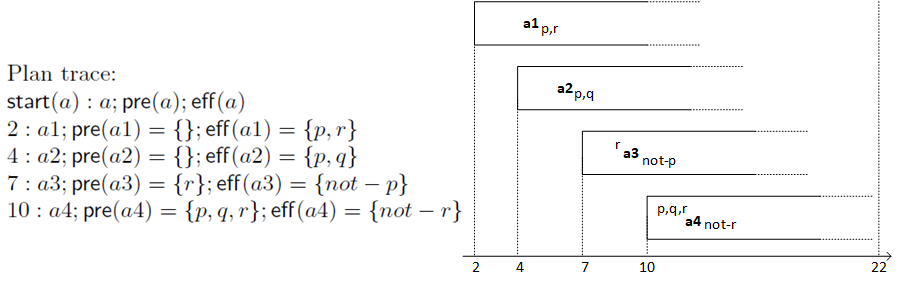
\includegraphics[width=12cm]{ejemploacciones2.png}
\caption{A simple example of how learning a temporal action model from $O$ and $A?$ is not straightforward. We (optionally) observe the plan makespan is 22.}
%, but depending on the distribution of conditions, effects and durations, many situations are possible, though some of them inconsistent.}
\label{fig:exampleplantrace}
\end{figure}


Let us suppose the example of Fig.~\ref{fig:exampleplantrace}, with all the start times, conditions and effects of actions. Clearly, $a3$ needs $a1$ to have $r$ supported, which represents the causal link or dependency $\tup{a1,r,a3}$. Let us imagine that $r$ is in $\cond_s(a3)$. In such a case, if $r$ is in $\eff_s(a1)$, $\dur(a1)$ is irrelevant to $a3$, but if $r$ is in $\eff_e(a1)$, $\dur(a1)$ has to be lower or equal than 5 ($\start(a1)+\dur(a1) \leq \start(a3)$). On the contrary, if $r$ is in $\cond_e(a3)$, $\dur(a1)$ could be much longer. Therefore, the distribution of conditions and effects has a significant impact in the durations, and vice versa.

$a4$ needs $p$, which means two possible causal links ($\tup{a1,p,a4}$ or $\tup{a2,p,a4}$). The real causal link will be the last to happen, and this depends on the effects+durations of $a1$ and $a2$. Therefore, the causal links are unknown, not easy to detect and they affect the structure of the temporal plan. But $a4$ really needs both $a1$ and $a2$ to have $p,q,r$ supported. Let us imagine that $p,q,r$ are in $\cond_s(a4)$ and $p,q$ in $\eff_e(a2)$; then $\dur(a2) \leq 6$. Even if we knew for sure that $\dur(a2)=6$ and $r$ was in $\eff_e(a1)$, we could never estimate the exact value of $\dur(a1)$, as any value in $]0..8]$ would be valid. Intuitively, an action has to wait until the last of its supports, but we cannot grant when the previous supports happen.%; those supporting times and respective durations can never be assured. 
Therefore, in some situations the precise duration cannot be found and we can only provide values that make the model consistent.

On the other hand, $a3$ deletes $p$, which means that it might \emph{threat} the causal link $\tup{a1,p,a4}$ or $\tup{a2,p,a4}$. But again, this threat depends on the distribution of conditions+effects and the durations. For instance, if $not-p$ is in $\eff_s(a3)$, then $a1$ or $a2$ must support $p$ after time 7 and before $a4$ requires it, which entails many consistent alternatives. On the contrary, if $p$ is in both $\eff_s(a1)$ and $\eff_s(a2)$, the observations on this plan trace are inconsistent as $a3$ deletes $p$ and no other action in the plan supports $p$ for $a4$. However, if $not-p$ is in $\eff_e(a3)$, $\dur(a3) > 3$ and $p$ is in $\cond_s(a4)$, then no threat will occur in the plan. Therefore, causal links and threats can easily appear or disappear depending on the selected distributions and durations.

Finally, there are some philosophical questions without a clearly motivated answer. First, why some conditions are modeled as \emph{at start} and others as \emph{over all}? In \texttt{drive-truck} of Fig.~\ref{fig:exampleactions2}, why \texttt{(driving ?d ?t)} is required throughout the entire action but \texttt{(link ?from ?to)} only at its beginning? Apparently, the link between the two locations should remain all over the driving. So is this a wrong decision of the human modeler?
Second, why some effects are modeled as \emph{at start} and others as \emph{at end}? In \texttt{board-truck}, why is \texttt{(not (empty ?t))} happening at start and \texttt{(driving ?d ?t)} at end? Could it be in the opposite way?
Third, what happens if one action requires/supports what it deletes (see $a4$ in Fig.~\ref{fig:exampleplantrace}, which might threat itself)? In such a case, the delete effect should happen later than its requirement/supporting.
Four, what happens if all effects are \emph{at start}? This makes little sense, as the duration of the actions would be undetermined and could potentially exceed the known plan horizon or makespan no matter the problem goals. In Fig.~\ref{fig:exampleplantrace}, if the effects of $a1$ and $a2$ are \emph{at start}, is it sensible to allow their durations to pass a hypothetical limit of 22? In other words, once all plan goals are achieved, can the actions be executed beyond the plan makespan or do they need to be cut off to such a value? This could potentially lead to an infinite number of models and overlapping situations, so it is not commonly accepted.

As can be noticed, learning a temporal action model is not simple, and many possible combinations are feasible provided they fit the constraints the model imposes. Therefore, formulating a CSP seems a promising approach to address this learning task.



\section{A CP Formulation to Learn Temporal Planning Models}
%One-Shot Learning of Temporal Action Models with Constraint Programming}
%Toni: este título es el del paper. No me termina de gustar como titulo de seccion...
%De hecho, esta formulacion sirve para tanto one-shot como multi-shot. Es una formulacion generica para modelos temporales
\label{sec:CPformulation}

Our approach is to create a CSP that includes all the constraints the learning task requires. This includes: i) the observations on the start times; ii) the actions' conditions, effects and durations; iii) the causal structure of the plan with all possible supports; and iv) mechanisms to avoid threats and possible contradictory effects. This formulation, inspired in the work by \cite{garrido2009constraint}, is solver-independent. This means that any off-the-shelf CSP solver that supports the expressiveness of our formulation, with binary and non-binary constraints, can be used.

%AQUI NO, QUE TODAVIA NO SE HAN INTRODUCIDO LAS VARS!!! First we introduce a temporal model formulation that is more expressive than PDDL2.1, and allows conditions and effects to be at any time, even outside the execution of the action. For instance, let us imagine a condition $p$ that only needs to be maintained for 5 time units before an action $a$ starts (e.g. warming-up a motor before driving): the expression $\reqe(p,a)=\start(a); \reqe(p,a) = \reqs(p,a)+5$ is possible in our formulation. Additionally, we can represent an effect $p$ that happens in the middle of action $a$: $\tim(p,a) = \start(a)+ (\dur(a) / 2)$ is also possible. The we present the formulation for PDDL2.1.


\subsection{The Variables}


For each action $a$ in $A?$, we create the seven kinds of variables specified in Table~\ref{table:variables}. Variables define the time-stamps for actions, the causal links, the interval when conditions must hold and the time when the effects happen. For simplicity, and to deal with integer variables, we model time in $\mathbb{Z}^+$. To prevent time from exceeding the plan horizon, we bound all times to the makespan of the plan.\footnote{We use the makespan, which can be observed, to restrict the duration of the actions. However, it is dispensable if we consider a long enough domain for durations}


\begin{table}
\begin{center}
\small
\begin{tabular}{p{2cm}p{2.7cm}p{7.4cm}}
Variable & Domain & Description \\

\hline

%\multicolumn{3}{l}{Vars. necessary for action times} \\

$\start(a)$ & \emph{known value} & start time of $a$ observed in $O$ \\
$\dur(a)$ & $[1..makespan]$ & duration of $a$. Optionally, it can be bounded by $makespan-\start(a)$\\
$\en(a)$ & \emph{derived value} & end time of $a$: $\en(a)=\start(a)+\dur(a)$ \\

%\multicolumn{3}{l}{Vars. necessary for action conditions+effects} \\

$\supp(p,a)$ & $\{b_i\}$ that \newline supports $p$ & symbolic variable for the set of potential supporters $b_i$ of condition $p$ of $a$ (causal link $\tup{b_i,p,a}$) \\

$\reqs(p,a)$, \\
$\reqe(p,a)$ & $[0..makespan]$ & interval $[\reqs(p,a)..\reqe(p,a)]$ at which action $a$ requires $p$ \\

$\tim(p,a)$ & $[0..makespan]$ & time when effect $p$ of $a$ happens \\


\hline
\end{tabular}
\normalsize
\end{center}
\caption{Formulation of variables and their domains for actions in $A?$.}
\label{table:variables}
\end{table}



Our temporal model formulation is more expressive than PDDL2.1 (see more details in section~\ref{sec:PDDL21constraints}), and allows conditions and effects to be at any time, even outside the execution of the action. For instance, let us imagine a condition $p$ that only needs to be maintained for 5 time units before an action $a$ starts (e.g. warming-up a motor before driving): the expression $\reqe(p,a)=\start(a); \reqe(p,a) = \reqs(p,a)+5$ is possible in our formulation. Additionally, we can represent an effect $p$ that happens in the middle of action $a$: $\tim(p,a) = \start(a)+ (\dur(a) / 2)$ is also possible.



Additionally, we create two dummy actions $\ini$ and $\goal$ for each planning problem $\tup{F,I,G,A}$. First, $\ini$ represents the initial state $I$ ($\start(\ini)=0$ and $\dur(\ini)=0$). $\ini$ has no variables $\supp, \reqs$ and $\reqe$ because it has no conditions. $\ini$ has as many $\tim(p_i,\ini)=0$ as $p_i$ in $I$. Second, $\goal$ represents $G$ ($\start(\goal)=makespan$ and $\dur(\goal)=0$). $\goal$ has as many $\supp(p_i,\goal)$ and $\reqs(p_i,\goal)=\reqe(p_i,\goal)=makespan$ as $p_i$ in $G$. $\goal$ has no variables $\tim$ as it has no effects.



%This formulation allows us to model TILs and observations exactly like other actions. On the one hand, $\til(f,t)$ can be seen as a dummy action ($\start(\til(f,t))=t$ and $\dur(\til(f,t))=0$) with no conditions and only one effect $f$ that happens at time $t$ ($\tim(f,\til(f,t))=t$). A $\til$ is analogous to $\ini$, as they both represent information that is given at a particular time, but externally to the execution of the plan. On the other hand, $\obs(f,t)$ can be seen as another dummy action ($\start(\obs(f,t))=t$ and $\dur(\obs(f,t))=0$) with only one condition $f$, which is the value observed for fact $f$, and no effects at all. An $\obs$ is analogous to $\goal$, as they both represent conditions that must be satisfied in the execution of the plan at a particular time.


\subsection{The Constraints}

Table~\ref{table:constraints} shows the constraints that we define among the variables of Table~\ref{table:variables}. The three first constraints are intuitive enough. The fourth constraint models the causal links. Note that in a causal link $\tup{b_i,p,a}$, $\tim(p,b_i) < \reqs(p,a)$ and not $\leq$. This is because temporal planning assumes an $\epsilon > 0$ as a small tolerance between the time when an effect $p$ is supported and when it is required~\cite{fox2003pddl2}. Since we model time in $\mathbb{Z}^+$, $\epsilon=1$ and $\leq$ becomes $<$.
The fifth constraint avoids any threat via promotion or demotion~\cite{ghallab2004automated}. The sixth constraint models the fact the same action requires and deletes $p$. Note the $\geq$ inequality here; this is possible because if one condition and one effect of $a$ happen at the same time, the underlying semantics in planning considers the condition is checked instantly before the effect~\cite{fox2003pddl2}. The seventh constraint solves the fact that two (possibly equal) actions have contradictory effects. It is important to note that these constraints involve any type of action, including $\ini$ and $\goal$.


%It is important to note that constraints involve any type of actions. Consequently, $\ini$, $\goal$, $\til$ and $\obs$ are subsumed in this formulation.



\begin{table}
\begin{center}
\small
\begin{tabular}{p{5cm}p{7.1cm}}
Constraint & Description \\

\hline

$\en(a)=\start(a)+\dur(a)$ & end time of $a$ \\

$\en(a) \leq \start(\goal)$ & $\goal$ is always the last action of the plan \\

%$\reqs(p,a) \leq \reqe(p,a)$ & [$\reqs(p,a)..\reqe(p,a)$] must be a valid interval \\
$\reqs(p,a) \leq \reqe(p,a)$ & interval [$\reqs(p,a)..\reqe(p,a)$] must be valid \\

\begin{tabular}{l}
if $\supp(p,a)=b_i$ then \\
\hspace{0.2cm}$\tim(p,b_i) < \reqs(p,a)$
\end{tabular}
& modeling causal link $\tup{b_i,p,a}$: the time when $b_i$ supports $p$ must be before $a$ requires $p$ \\

\begin{tabular}{l}
$\forall b_j \neq a$ that deletes $p$ at time $\tau_j$: \\
\hspace{0.2cm}if $\supp(p,a)=b_i$ then \\
\hspace{0.4cm}$\tau_j < \tim(p,b_i)$ OR \\
\hspace{0.4cm}$\tau_j > \reqe(p,a)$
\end{tabular}
& solving threat of $b_j$ to causal link $\tup{b_i,p,a}$ being $b_j \neq a$ (promotion OR demotion)\\

\begin{tabular}{l}
if $a$ requires and deletes $p$: \\
\hspace{0.2cm}$\tim(not-p,a) \geq \reqe(p,a)$ \\
\end{tabular}
& when $a$ requires and deletes $p$, the effect cannot happen before the condition \\

\begin{tabular}{l}
$\forall a_i,a_j \mid a_i$ supports $p$ and \\
\hspace{1.2cm}$a_j$ deletes $p$: \\
\hspace{0.2cm}$\tim(p,a_i) \neq \tim(not-p,a_j)$ \\
\end{tabular}
& solving effect interference ($p$ and $not-p$): they cannot happen at the same time \\

\hline
\end{tabular}
\normalsize
\end{center}
\caption{Formulation of constraints.}
\label{table:constraints}
\end{table}



\subsection{Specific Constraints for Durative Actions of PDDL2.1}
\label{sec:PDDL21constraints}

As section~\ref{sec:temporalplanning} explains, PDDL2.1 restricts the expressiveness of temporal planning in terms of conditions, effects, durations and structure of the actions. Hence, our temporal formulation subsumes and is significantly richer than PDDL2.1; but adding constraints to make it fully PDDL2.1-compliant is straightforward.


First, adding $((\reqs(p,a) = \start(a))$ OR ($\reqs(p,a) = \en(a)))$ AND $((\reqe(p,a) = \start(a))$ OR ($\reqe(p,a) = \en(a)))$ limits condition $p$ to be \emph{at start}, \emph{over all} or \emph{at end}, i.e. $p$ is in $\cond_s(a)$, $\cond_o(a)$ or $\cond_e(a)$, respectively.
Further, if a condition is never deleted in a plan, it can be considered as an invariant condition for such a plan. In other words, it represents static information. This type of condition is commonly used in planning to ease the grounding process from the operators; e.g. to model that there is a link between two locations and, consequently, a driving is possible, or modeling a petrol station that allows a refuel action in a given location, etc. Therefore, the constraint to be added for an invariant condition $p$ is simply: $((\reqs(p,a) = \start(a))$ AND $(\reqe(p,a) = \en(a)))$, i.e. $p \in \cond_o(a)$.
Surprisingly, invariant conditions are modeled differently depending on the human modeler. See, for instance, \texttt{(link ?from ?to)} of Fig.~\ref{fig:exampleactions2}, which is modeled as an \emph{at start} condition despite: i) the link should be necessary all over the driving, and ii) no action in this domain can be planned to delete that link.
This also happens in the \emph{transport} domain of the IPC, where a refuel action requires to have a petrol station in a location only \emph{at start}, rather than \emph{over all} which makes more sense. This shows that modeling a planning domain is not easy and it highly depends on the human's decision. On the contrary, our formulation checks the invariant conditions and deals with them always in the same coherent way.


Second, $((\tim(p,a) = \start(a))$ OR $(\tim(p,a) = \en(a)))$ makes an effect $p$ happen only \emph{at start} or \emph{at end} of action $a$, i.e. $p$ is in $\eff_s(a)$ or $\eff_e(a)$.
Also, if all effects happen \emph{at start} the duration of the action would be irrelevant and could exceed the plan makespan. To avoid this, for any action $a$, at least one of its effects should happen \emph{at end}: $\sum_{i=1}^{n =|\eff(a)|} \tim(p_i,a) > n \cdot \start(a)$, which guarantees $\eff_e(a)$ is not empty.

%\begin{displaymath}
%\sum_{i=1}^{n = \textrm{number of effects of }a} \tim(p_i,a) > n \cdot \start(a)
%\end{displaymath}


Third, durations in PDDL2.1 can be defined in two different ways. On the one hand, durations can be equal for all grounded actions of the same operator. For instance, any instantiation of \texttt{board-truck} of Fig.~\ref{fig:exampleactions2} will last 2 time units no matter its parameters. Although this may seem a bit odd, it is not an uncommon practice to simplify the model. The constraint to model this is: $\forall a_i,a_j$ being instances of the same operator: $\dur(a_i) = \dur(a_j)$.
On the other hand, although different instantiations of \texttt{drive-truck} will last different depending on the locations, different occurrences of the same instantiated action will last equal.
In a PDDL2.1 temporal plan, multiple occurrences of \texttt{drive-truck(truck1,loc1,loc2,driver1)} will have the same duration no matter when they start. Intuitively, they are different occurrences of the same action, but in the real-world the durations would differ from driving at night or in peak times. Since PDDL2.1 makes no distinction among different occurrences, the constraint to add is: $\forall a_i,a_j$ being occurrences of the same durative action: $\dur(a_i) = \dur(a_j)$.
Obviously, this second constraint is subsumed by the first one in the general case where all instances of the same operator have the same duration.

Fourth, the structure of conditions and effects for all grounded actions of the same operator is constant in PDDL2.1. This means that if \texttt{(empty ?t)} is an \emph{at start} condition of \texttt{board-truck}, it will be \emph{at start} in any of its grounded actions.
Let $\{p_i\}$ be the conditions of an operator and $\{a_j\}$ be the instances of a particular operator. The following constraints are necessary to guarantee a constant structure:

$\forall p_i: (\forall a_j: \reqs(p_i,a_j) = \start(a_j))$ OR $(\forall a_j: \reqs(p_i,a_j) = \en(a_j))$

$\forall p_i: (\forall a_j: \reqe(p_i,a_j) = \start(a_j))$ OR $(\forall a_j: \reqe(p_i,a_j) = \en(a_j))$

And analogously for all effects $\{p_i\}$ and the instances $\{a_j\}$ of an operator:

$\forall p_i: (\forall a_j: \tim(p_i,a_j) = \start(a_j))$ OR $(\forall a_j: \tim(p_i,a_j) = \en(a_j))$


As a conclusion, in our formulation each action of $A?$ is modeled separately so it does not need to share the same structure or duration of other actions. Moreover, the time-stamps for conditions/effects can be arbitrarily placed inside or outside the execution of the action, which allows for a flexible and expressive temporal model. But, when necessary, we can simply include additional constraints to restrict the expressiveness of the model, such as the ones provided by PDDL2.1.


\subsection{Example}
\label{sec:example}

We now show a fragment of the formulation for the example depicted in Fig.~\ref{fig:exampleplantrace}. For simplicity, we only show the variables and constraints for action $a3$, but the formulation is analogous for all other actions.

The variables and domains are: $\start(a3)=7$; $\dur(a3) \in [1..15]$; $\en(a3)=\start(a3)+\dur(a3)$; $\supp(r,a3) \in \{a1\}$; $\reqs(r,a3),\reqe(r,a3) \in [0..22]$; and $\tim(not-p,a3) \in [0..22]$.
On the other hand, the constraints are: $\en(a3) \leq \start(\goal)$; $\reqs(r,a3) \leq \reqe(r,a3)$; if $\supp(r,a3)=a1$ then $\tim(r,a1) < \reqs(r,a3)$; if $\supp(r,a3)=a1$ then $((\tim(not-r,a4) < \tim(r,a1))$ OR $(\tim(not-r,a4) > \reqe(r,a3)))$; $\tim(not-p,a3) \neq \tim(p,a1)$ and $\tim(not-p,a3) \neq \tim(p,a2)$.

There are many consistent solutions for this simple example, mainly because there is a huge range of possible durations that make the learned model consistent with the partially specified model $A?$.
Fig.~\ref{figure:solutionsExample} shows six arbitrary models as solutions. What is important to note is that the structure, i.e. distribution of conditions/effects, is similar in all the learned models. Actually, the distribution of the effects is identical (except for $q$ in model 2), and the distribution of conditions is very similar (e.g. $q$ is always in $\cond_o$ and $r$ in $a4$ is very often in $\cond_o$).
This shows that the one-shot learning returns not only consistent models but also similar, which is very positive.
The durations are, however, more different: $\dur(a1)$ ranges in these models from 7 to 19, whereas $\dur(a2)$ ranges from 5 to 18. As explained in section~\ref{sec:simpleTask}, learning the precise duration from just one sample may not be always possible, which is the main limitation of the one-shot learning task.
%Clearly, the duration learned for only one sample of \texttt{drive-truck(truck1,loc1,loc2,driver1)} cannot be always generalized to any other driving between these two locations.
In fact, the specific constraint of PDDL2.1, with regard to having multiple occurrences of the same action having the same duration, can significantly help us to learn the actions' duration in a more precise way as the learned duration must be consistent with all those occurrences.


\begin{figure}
\footnotesize
\begin{tabular}{ll}
\hspace{-0.6cm}\begin{tabular}{lllllll}
Action & $\dur$ & $\cond_s$ & $\cond_o$ & $\cond_e$ & $\eff_s$ & $\eff_e$ \\

\hline

\multicolumn{7}{l}{Learned model 1} \\
$a1$ & 8 & & & & $r$ & $p$ \\
$a2$ & 18 & & & & $q$ & $p$ \\
$a3$ & 1 & & $r$ & & & $not-p$ \\
$a4$ & 1 & & $q,r$ & $p$ & & $not-r$ \\

\hline

\multicolumn{7}{l}{Learned model 2} \\
$a1$ & 19 & & & & $r$ & $p$ \\
$a2$ & 5 & & & & & $p,q$ \\
$a3$ & 1 & & & $r$ & & $not-p$ \\
$a4$ & 1 & $r$ & $p,q$ & & & $not-r$ \\

\hline

\multicolumn{7}{l}{Learned model 3} \\
$a1$ & 7 & & & & $r$ & $p$ \\
$a2$ & 18 & & & & $q$ & $p$ \\
$a3$ & 1 & & & $r$  & & $not-p$ \\
$a4$ & 1 & & $p,q,r$ & & & $not-r$ \\
\end{tabular} &

\hspace{0.3cm}\begin{tabular}{lllllll}

Action & $\dur$ & $\cond_s$ & $\cond_o$ & $\cond_e$ & $\eff_s$ & $\eff_e$ \\

\hline

\multicolumn{7}{l}{Learned model 4} \\
$a1$ & 7 & & & & $r$ & $p$ \\
$a2$ & 9 & & & & $q$ & $p$ \\
$a3$ & 1 & & & $r$ & & $not-p$ \\
$a4$ & 1 & & $p,q,r$ & & & $not-r$ \\

\hline

\multicolumn{7}{l}{Learned model 5} \\
$a1$ & 9 & & & & $r$ & $p$ \\
$a2$ & 6 & & & & $q$ & $p$ \\
$a3$ & 1 & & $r$ & & & $not-p$ \\
$a4$ & 1 & & $q,r$ & $p$ & & $not-r$ \\

\hline

\multicolumn{7}{l}{Learned model 6} \\
$a1$ & 8 & & & & $r$ & $p$ \\
$a2$ & 16 & & & & $q$ & $p$ \\
$a3$ & 1 & $r$ & & & & $not-p$ \\
$a4$ & 1 & & $q,r$ & $p$ & & $not-r$ \\

\end{tabular} \\

\end{tabular}
\normalsize

\caption{Six learned models for the example of Fig.~\ref{fig:exampleplantrace}, but there are many more.}
\label{figure:solutionsExample}
\end{figure}


%\subsection{Properties}

%Soundness of our formulation is guaranteed by the definition of the constraints of Table~\ref{table:constraints}, where all the branching alternatives to solve causal links, threats and effect interferences are supported. Completeness is guaranteed by the complete exploration of the domain of each variable of Table~\ref{table:variables} which can return many learned models in the form of consistent alternative solutions.



\subsection{Implementation. Use of Heuristics for Resolution}
\label{sec:implementation}

Our CSP formulation is automatically compiled from a partially specified action model, as defined in a classical planning problem, and the observations from a plan execution.
The formulation has been implemented in \textsf{Choco}\footnote{\texttt{http://www.choco-solver.org}}, an open-source Java library for constraint programming that provides an object-oriented API to state the constraints to be satisfied.

Our formulation is solver-independent, which means we do not use heuristics that may require changes in the implementation of the CSP engine.
Although this reduces the solver performance, we are interested in using it as a blackbox that can be easily changed with no modification in our formulation. However, we can easily encode standard static heuristics for variable and value selection that help improve efficiency by following the next ordering, which has shown very efficient in our experiments:

%%IMPORTANTE: ahorramos espacio juntando en la viñeta el orden de seleccion de variables y de valores

%From the variable perspective, we have detected it is better to instantiate variables that first lead to failure: effects, conditions, supporters and durations. This implies this ordering: $\tim$, $\reqs$, $\reqe$, $\supp$ and $\dur$.
%From the value perspective, we select first the values that lead to a more reasonable model of actions:

\begin{enumerate}
  \item Effects ($\tim$). For negative effects, first the lower value and for positive effects, first the upper value. This gives priority to delete effects as $\eff_s(a)$ and positive effects as $\eff_e(a)$.
  \item Conditions ($\reqs$ and $\reqe$). For $\reqs$, first the lower value, whereas for $\reqe$, first the upper value. This gives priority to $\cond_o(a)$, trying to keep the conditions as long as possible.
  \item Supporters ($\supp$). First the lower value, thus preferring the supporter that starts earlier in the plan.
  \item Duration ($\dur$). First the lower value, thus applying the principle of the shortest actions that make the learned model consistent.
\end{enumerate}


%This simple collection of heuristics is very intuitive and has been used in \textsf{Choco} by simply overriding the default search strategy for the variable and value selectors. Although these heuristics have shown very efficient in our experiments, they cannot always guarantee the best performance.


\subsection{Using the CP Formulation for Plan Validation}
\label{sec:usingCPValidation}

%As seen above, adding constraints allows us to restrict the temporal expressiveness of the learned model.
We explained that adding extra constraints allows us to restrict the temporal expressiveness of the learned model. We show here that we can also restrict the learned model by constraining the variables to known values, which is specially interesting when there is additional information on the temporal model that needs to be represented. For instance, based on past learned models, we may know the precise duration of an action $a$ is 6,
%or we can figure out that a condition is a start condition
or we can figure out that an effect $p$ always happens at end.
Our CP formulation can include this by simply adding $\dur(a)=6$ and $\tim(p,a)=\en(a)$, respectively, which is useful to enrich the partially specified actions in $A?$ of the learning task.

%The CP formulation is also useful to validate whether a given action model is consistent, as we will see in section~\ref{sec:evaluation}.
In particular, the possibility of adding those constraints is very appealing when used for validating whether a partial action model allows us to learn a consistent model, as we will see in section~\ref{sec:evaluation}.
Let us assume that the distribution of all (or just a few) conditions and/or effects is known and, in consequence, represented in the learning task. If a solution is found, then that structure of conditions/effects is consistent for the learned model. On the contrary, if no solution is found that structure is inconsistent and cannot be explained.
Analogously, we can represent known values for the durations. If a solution is found, the durations are consistent, and inconsistent otherwise.
Hence, we have three options for validating a partial model \emph{w.r.t.}: i) a known structure with the distribution of conditions/effects; ii) a known set of durations; and iii) a known structure plus a known set of durations (i+ii).
The first and second option allows for some flexibility in the learning task because some variables remain open. On the contrary, the third option checks whether a learned model can fit the given constraints, thus reproducing a strict plan validation task equivalent to~\cite{howey2004val}.



\section{Evaluation}
\label{sec:evaluation}

\subsection{Evaluation Metrics}


The empirical evaluation of a learning task can be addressed from two perspectives. From a pure syntactic perspective, learning can be considered as an automated design task to create a new model that is similar to a reference (or {\em ground truth}) model. Consequently, the success of learning is an accuracy measure of how similar these two models are, which usually counts the number of differences (in terms of incorrect durations or distribution of conditions/effects).
Unfortunately, there is not a unique reference model when learning temporal models at real-world problems.
Also, a pure syntax-based measure usually returns misleading and pessimistic results, as it may count as incorrect a different duration or a change in the distribution of conditions/effects that really represent equivalent reformulations of the reference model. For instance, given the example of Fig.~\ref{fig:exampleactions2}, the condition learned \texttt{(over all (link ?from ?to))} would be counted as a difference in action \texttt{drive-truck}, as it is \texttt{at start} in the reference model; but it is, semantically speaking, even more correct. Analogously, some durations may differ from the reference model but they should not be counted as incorrect. As seen in section~\ref{sec:simpleTask}, some learned durations cannot be granted, but the underlying model is still consistent. Therefore, performing a syntactic evaluation in learning is not always a good idea.


From a semantic perspective, learning can be considered as a classification task where we first learn a model from a training dataset, then tune the model on a validation test and, finally, asses the model on a test dataset. Our approach represents a one-shot learning task because we only use one plan sample to learn the model and no validation step is required.
Therefore, the success of the learned model can be assessed by analyzing the success ratio of the learned model \emph{vs.} all the unseen samples of a test dataset. In other words, we are interested in learning a model that fits as many samples of the test dataset as possible. This is the evaluation that we consider most valuable for learning, and define the success ratio as the percentage of samples of the test dataset that are consistent with the learned model. A higher ratio means that the learned model explains, or adequately fits, the observed constraints the test dataset imposes.


\subsection{Experimental Results}

%569 instances on nine IPC planning domains
We have run experiments on nine IPC planning domains. It is important to highlight that these domains are encoded in PDDL2.1, with the number of operators shown in Table~\ref{table:evaluationExperiments}, so we have included the constraints given in section~\ref{sec:PDDL21constraints}. We first get the plans for these domains by using five planners (\textit{LPG-Quality}~\cite{gerevini2003planning}, \textit{LPG-Speed}~\cite{gerevini2003planning}, \textit{TP}~\cite{jimenez2015temporal}, \textit{TFD}~\cite{eyerich2009using} and \textit{TFLAP}~\cite{marzal2016temporal}), where the planning time is limited to 100s.
The actions and observations on each plan are automatically compiled into a CSP learning instance. Then,
%we create the CP formulation and
we run the one-shot learning task to get a temporal action model for each instance, where the learning time is limited to 100s on an Intel i5-6400 @ 2.70GHz with 8GB of RAM.
In order to assess the quality of the learned model, we validate each model \emph{vs.} the other models \emph{w.r.t.} the \emph{struct}ure, the \emph{dur}ation and the \emph{struct}ure+\emph{dur}ation, as discussed in section~\ref{sec:usingCPValidation}.
For instance, the \emph{zenotravel} domain contains 78 instances, which means learning 78 models. Each model is validated by using the 77 remaining models, thus producing 78$\times$77=6006 validations per struct, dur and struct+dur each. The value for each cell is the average success ratio.
In \emph{zenotravel}, the struct value means that the distribution of conditions/effects learned by using only one plan sample is consistent with all the samples used as dataset (100\% of the 6006 validations), which is the perfect result, as also happens in \emph{floortile} and \emph{sokoban} domains.
The dur value means the durations learned explain 68.83\% of the dataset. This value is usually lower because any learned duration that leads to inconsistency in a sample counts as a failure. The struct+dur value means that the learned model explains entirely 35.76\% of the samples. This value is always the lowest because a subtle structure or duration that leads to inconsistency in a sample counts as a failure.
As seen in Table~\ref{table:evaluationExperiments}, the results are specially good, taking into consideration that we use only one sample to learn the temporal action model.
These results depend on the domain size (number of operators, which need to be grounded), the relationships (causal links, threats and interferences) among the actions, and the size and quality of the plans.



\begin{table}
\begin{center}
\small
%\begin{tabular}{p{2cm}p{2cm}p{1cm}p{1cm}p{2cm}}
\begin{tabular}{p{2cm}ccccc}
Domain & No. operators & No. instances & struct & dur & struct+dur  \\

\hline

\emph{zenotravel} & 5 & 78 & 100\% & 68.83\% & 35.76\% \\
\emph{driverlog} & 6 & 73 & 97.60\% & 44.86\% & 21.04\% \\
\emph{depots} & 5 & 64 & 55.41\% & 76.22\% & 23.19\% \\
\emph{rovers} & 9 & 84 & 78.84\% & 5.35\% & 0.17\% \\
\emph{satellite} & 5 & 84 & 80.74\% & 57.13\% & 40.53\% \\
\emph{storage} & 5 & 69 & 58.08\% & 70.10\% & 38.36\% \\
\emph{floortile} & 7 & 17 & 100\% & 80.88\% & 48.90\%\\

\emph{parking} & 4 & 49 & 86.69\% & 81.38\% & 54.89\% \\
\emph{sokoban} & 3 & 51 & 100\% & 87.25\% & 79.96\% \\

\hline
\end{tabular}
\normalsize
\end{center}
\caption{Average success ratio of the one-shot learned model \emph{vs.} the test dataset in different IPC planning domains.}
\label{table:evaluationExperiments}
\end{table}


We have observed that some planners return plans with unnecessary actions, which has a negative impact for learning precise durations.
%Some planners return plans with unnecessary actions, thus making an adequate learning more difficult. In particular, actions that are redundant have a negative impact for learning precise durations.
The worst result is returned in the \emph{rovers} domain, which models a group of planetary rovers to explore the planet they are on. Since there are many parallel actions for taking pictures/samples and navigation of multiple rovers, learning the duration and the structure+duration is particularly complex in this domain.



%\section{Discussion}
%\label{sec:discussion}

%Indicar que cambios hace falta para que un cp-planner pueda actuar como learner/validator.


\section{Conclusions}
\label{sec:conclusions}


We have presented a purely declarative CP formulation, which is independent of any CSP solver, to address the learning of temporal action models. Learning in planning is specially interesting to recognize past behavior in order to predict and anticipate actions to improve decisions.
The main contribution is a simple formulation that is automatically derived from the actions and observations on each plan execution, without the necessity of specific hand-coded domain knowledge. It is also flexible to support a very expressive temporal planning model, though it can be easily modified to be PDDL2.1-compliant.
Formal properties are inherited from the formulation itself and the CSP solver. The formulation is correct because the definition of constraints to solve causal links, threats and effect interferences are supported, which avoids contradictions. It is also complete because the solution needs to be consistent with all the imposed constraints, while a complete exploration of the domain of each variable returns all the possible learned models in the form of alternative consistent solutions.


Unlike other approaches that need to learn from datasets with many samples, we perform a one-shot learning. This reduces both the size of the required datasets and the computation time. The one-shot learned models are very good and explain a high number of samples in the datasets used for testing. Moreover, the same CP formulation is valid for learning and for validation, by simply adding constraints to the variables. This is an advantage, as the same formulation allows us to carry out different tasks: from entirely learning, partial learning/validation (structure and/or duration) to entirely plan validation.
According to our experiments, learning the structure of the actions in a one-shot way leads to representative enough models, but learning the precise durations is more difficult, and even impossible, when many actions are executed in parallel.


Finally,
%it is important to note that
our CP formulation can be represented and solved by Satisfiability Modulo Theories, which is part of our current work. As future work, we want to extend our formulation to learn meta-models, as combinations of many learned models, and a more complete action model.
In the latter, rather than using a partially specified set of actions, we want to find out the conditions/effects together with their distribution.
%We aim at finding out the conditions/effects together with their distribution, thus removing constraints from the partially specified set of actions in $A?$.
The underlying idea of finding an action model consistent with all the constraints will remain the same, but the model will need to be extended with additional decision variables and constraints. %$\mathsf{is\_condition(p,a)}$, $\mathsf{is\_effect(p,a)}$ to decide whether $p$ is a condition or effect of action $a$.
This will probably lead to the analysis of new heuristics for resolution.




%Finally,
%it is important to note that
%our CP formulation can be also represented and solved by Satisfiability Modulo Theories, which is part of our current work. As future work, we want to extend our formulation to learn a meta-model, as a combination of many learned models, and a more complete action model. In the latter, rather than using a partially specified set of actions in $A?$, we want to find out the conditions/effects together with their distribution.
%We aim at finding out the conditions/effects together with their distribution, thus removing constraints from the partially specified set of actions in $A?$.
%The underlying idea of finding an action model consistent with all the constraints will remain the same, but the model will need to be extended with additional constraints and decision variables $\mathsf{is\_condition(p,a)}$, $\mathsf{is\_effect(p,a)}$ to decide whether $p$ is a condition or effect of action $a$. This will probably lead to new heuristics for resolution.




%
% ---- Bibliography ----
%
% BibTeX users should specify bibliography style 'splncs04'.
% References will then be sorted and formatted in the correct style.
%
\bibliographystyle{splncs04}
\bibliography{tmodeling}
%
%\begin{thebibliography}{8}
%\end{thebibliography}
\end{document}



%We use the same model of action to represent all elements of temporal planning, including TILs and observations.
%The timed initial literals can be interpreted as simple actions that are forced into the respective happenings (rather than selected into them by the planner), whose precondition is true, and whose only effect is the respective literal.


Temporal planning in PDDL2.1 is not expressive enough, but our model allows us to represent higher levels of expressiveness.



“Approximate” domain models are those that are almost
complete, but have some missing details. Examples of
missing details could include missing preconditions and
effects of actions, or cost models. We would
like to be able to use approximate models to support plan
creation as well as plan critiquing. \cite{kambhampati2007model}



better-valued goals or
recommendation of alternative plans that report higher utility to the users (tourism). In
particular, the key idea is to use the generated models in automated planning, so as to propose
the agent what to do, how to do something or how to do it differently.



can be used in different real-world applications: helping elders or generic tasks;
to help smart cities decision making; decision support systems in e-Health, logistics, tourism, transportation, data-mining or e-learning


We are
interested in environments where observed data is regarded as sequences of activities and
thus provide helpful insight to intelligent assistants (domotics, or robotics for helping aging
people), decision making in smart cities (traffic), suggesting better-valued goals or
recommendation of alternative plans that report higher utility to the users (tourism). In
particular, the key idea is to use the generated models in automated planning, so as to propose
the agent what to do, how to do something or how to do it differently.



analyze information from sensors in order to generate diverse models of an
agent’s behavior, such as planning domain models, probabilistic models, or generic classifiers.




such as home
automation, where the system will learn about the habits and behavior of the inhabitants, it
will recognize critical situations and will suggest executing specific actions to avoid criticality
or focus on a different goal. In general,






IMPORTANTE: consistent with the sequence of observations, in order to select the hypothesis that best explains the
observations. The intuition behind inverse-planning-based approaches is that, given a sequence of
observations and a set of possible goals, the most likely goal to be pursued by an agent is the one which optimal plan is most consistent with the given observations


learning planning models from partial (incomplete) observability




Para related work ver: memoria Learning action models (pag 12)

